\chapter{Proposta} \label{cap:cap4}

A proposta de uso do dispositivo háptico para treinamento de anestesia raquidiana apresentada nesta tese envolve a criação de um simulador que permite o treinamento de aprendizes na técnica de anestesia raquidiana utilizando um ambiente virtual de treinamento.
Este ambiente virtual foi desenvolvido utilizando o motor de jogo Unity3D \cite{UnityTechnologies2020} com uso de \textit{plugin} para o dispositivo háptico \textit{Geomagic Touch}®, os \textit{scripts} foram desenvolvidos em C\#. O código foi desenvolvido como uma evolução do simulador epidural desenvolvido por \textcite{Brazil2017} levando em consideração que diversas funcionalidades existentes foram estendidas e modificadas assim como outras foram criadas. O foco passou de anestesia epidural para anestesia raquidiana. Um novo modelo 3D foi construído para representar fielmente as camadas do corpo humano, para isto, as formas e volumes das camadas foram baseadas num corpo 3D interativo cientificamente preciso \cite{BioDigitalInc2019}. Adicionalmente a isto as principais camadas (tecidos do corpo) foram programadas com um margem de crescimento individual onde o crescimento da camada mais interna "empurra" as camadas mais externas pra fora. Isto foi feito para possibilitar uma maior variabilidade de cenários e para que estes sejam visualmente coerentes quando a transparência das camadas for aplicada. Além da possibilidade de se crescer individualmente cada camada, também é possível que todas as camadas cresçam de forma homogênea através da aplicação de matrizes de transformação. 

\section {Desenvolvimento do ambiente de treinamento} 

O modelo 3D para o tronco do corpo feminino (área onde é feita a punção) foi desenvolvido usando o software de modelagem e criação \textit{3ds Max} \cite{Autodesk}. Exemplos das suas diversas camadas internas podem ser observados na figura \ref{fig:modelo3Dcorpo}. 

\begin{figure}[ht!]
    \centering
        \begin{tabular}{cc}
        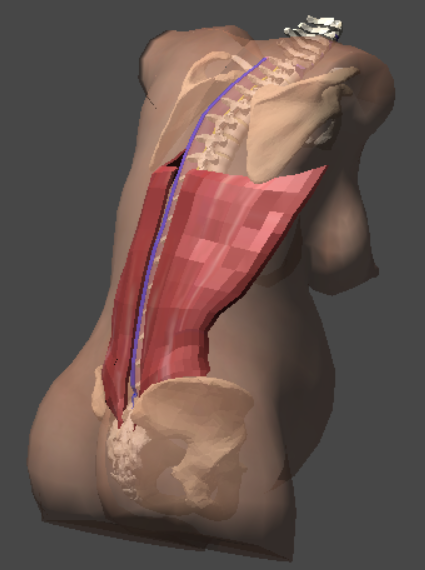
\includegraphics[width=0.4\linewidth]{capitulos/figuras/modelo corpo 3d.PNG} & 
        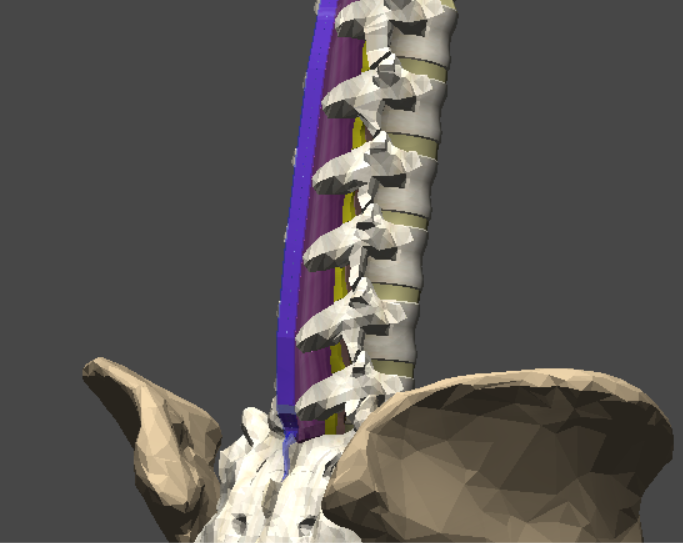
\includegraphics[width=0.6\linewidth]{capitulos/figuras/modelo corpo 3d - coluna vertebral, ligamentos supra, interespinhoso and flavum.PNG} 
        \\
        (a) & (b)
        \end{tabular}
    \caption{Modelo 3D de corpo de mulher grávida desenvolvido com diferentes níveis de transparência \cite{Melo2021}: (a) Corpo, ossos e músculos (b) Osso, vértebras e ligamentos.}
    \label{fig:modelo3Dcorpo}
\end{figure}

Como comentado anteriormente foram criados controles para crescimento das principais camadas do corpo. Para seu uso, primeiro é necessário iniciar um projeto na \textit{Unity} e importar o modelo 3D. Com isto estes controles ficam acessíveis via código nas diversas linguagens suportadas pela \textit{Unity} assim como via interface da \textit{Unity}. Para a nossa solução onde precisávamos fazer modificações em tempo de execução optamos pelo acesso através do código em C\# para fazer as modificações de tamanho das camadas (quando necessário). 

Para que seja possível fazer a interação com o dispositivo háptico \textit{Geomagic Touch®} o driver \textit{Open Haptics Touch Device} precisa ser instalado na máquina onde o dispositivo será usado, este driver pode ser encontrado no endereço eletrônico da empresa responsável pela produção e comercialização deste dispositivo háptico \cite{3DSystemsTouch2018}. Para que este dispositivo possa ser utilizado na \textit{Unity} optamos pela instalação do \textit{Haptic Plug-In For Unity3D} \cite{Poyade2014}. Este \textit{plugin} contém exemplos que exploram as funcionalidades e dos dispositivos hápticos suportados. As características específicas que foram utilizadas nos experimentos são comentadas no capítulo~\ref{cap:cap5}. No ambiente de treinamento utilizamos configurações similares as dos experimentos ajustadas de acordo com cada corpo de paciente sendo simulado. 

Foi incluída uma visão lateral da cena (Figura~\ref{fig:posicaoSentadaComTransparencia}) a partir do \textit{feedback} de um anestesista sobre pontos de melhoria da ferramenta de treinamento para possibilitar um outro ponto de vista do procedimento sendo efetuado. Esta característica ajuda não só o indivíduo em treinamento mas também pessoas que possam assistir o treinamento ao vivo ou ainda gravações deste que pode ser disponibilizado futuramente. Nesta mesma imagem fizemos também a demonstração da visibilidade das camadas interiores do corpo (que é exibida ao pressionar usando o mouse o botão "visibilidade" no menu do lado esquerdo). Esta funcionalidade pode ser utilizada por iniciantes nos seus primeiros treinamentos assim como por educadores para turmas que estejam assistindo demonstrações feita por estes.  

\begin{figure}[ht!]
    \centering
    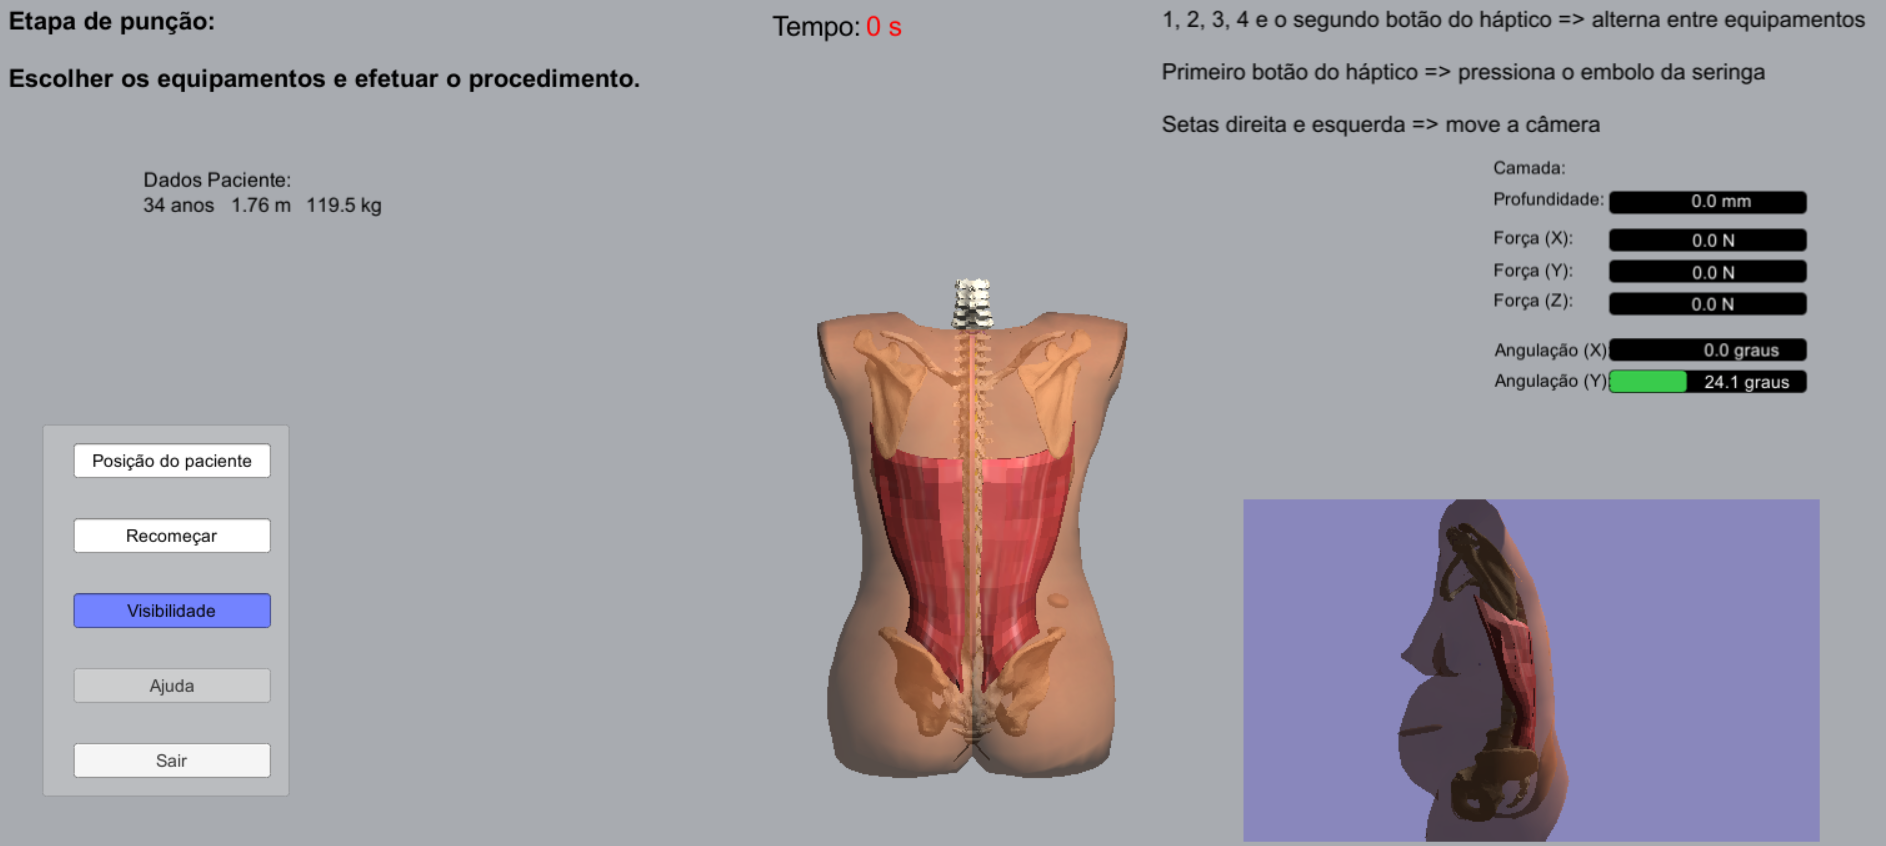
\includegraphics[width=0.9\linewidth]{capitulos/figuras/sistema posicao sentada com transparencia.png} 
    \caption{Visão geral do sistema com tronco de paciente centralizada na tela na posição sentada. Do lado inferior direito a visão lateral desta mesma parte do corpo. Neste caso foi aplicada a transparência para visualização das camadas internas}
    \label{fig:posicaoSentadaComTransparencia}
\end{figure}

Uma outra opção de execução do procedimento incluída foi a possibilidade de mudança de posição da paciente (Figura~\ref{fig:posicaoDeitada}) que além da posição sentada (original e mais comum) agora também permite que o procedimento seja feito com ela deitada (estas são as duas posições em que ocorre o procedimento de raquianestesia \ref{sec:anestesiaRaquidiana}).

\begin{figure}[ht!]
    \centering
    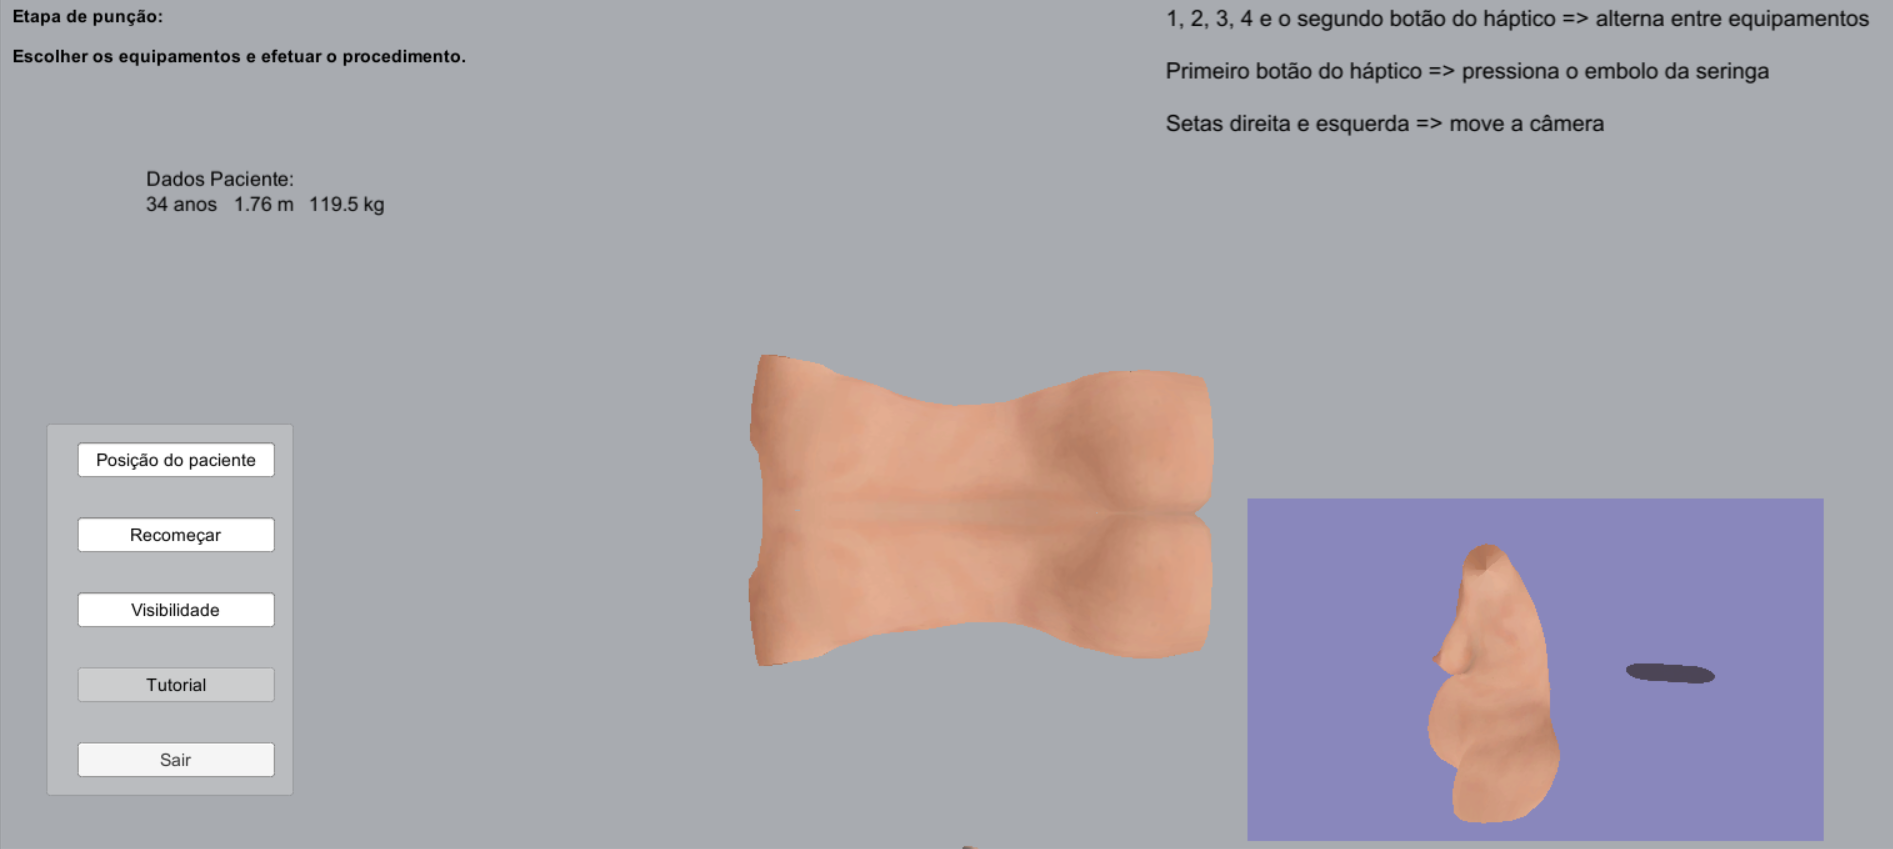
\includegraphics[width=0.9\linewidth]{capitulos/figuras/sistema posicao deitada.png} 
    \caption{Visão geral do sistema com tronco de paciente na posição deitada.}
    \label{fig:posicaoDeitada}
\end{figure}

\subsection {Simulação de pacientes virtuais} 
\label{sec:SimulacaoPacientesVirtuais}

Um dos benefícios da criação de ambientes virtuais para treinamento é a possibilidade de se ter uma quantidade muito grande de casos para o treinamento. Estas possibilidades estão limitadas somente pela abrangência do modelo para criação de pacientes virtuais. Conforme descrito anteriormente para esta tese foi criado e utilizado um modelo dinâmico para geração de pacientes do sexo feminino grávidas. A variação física externamente visível das pacientes é função da altura e massa corpórea. Para as camadas internas envolvidas na anestesia raquidiana a \acrlong{DEE} (\acrshort{DEE}) também entra nessa conta para uma representação mais real da distância entre estas camadas conforme descrito na seção \ref{sec:modelagemTecidos}. 

============================================

Iniciamos esta seção descrevendo como fizemos o uso dos dados e equações de populações locais descritas por \textcite{Clinkscales2007, Sharma2011, Hazarika2016} para a modelagem de uma equação mais geral na determinação da \acrshort{DEE}. A abordagem que detalharemos aqui foi uma das duas abordagens descritas em trabalho publicado por nós \cite{Melo2020}.
Como os dados brutos das populações dos três trabalhos analisados não foram disponibilizados publicamente, utilizamos os dados das equações disponibilizadas para gerar pacientes representativos de cada população.

Como \textcite{Sharma2011} ao invés das equações apresentaram a \acrshort{DEE} estimada para cada grupo populacional optamos por Utilizar o método dos mínimos quadrados para obter as equações de cada grupo através do melhor ajuste de curva que representasse cada um dos quatro grupos da Tabela~\ref{tab:DEEEstimadosSharma}. Para cada ponto consideramos o eixo X como \acrshort{IMC} e o eixo Y como a \acrshort{DEE} estimada. As equações resultado para cada grupo desta tabela que minimiza a soma do quadrado das diferenças para cada ponto está descrito nas equações presentes na Tabela~\ref{tab:DEEEquacoesMinimosQuadrados}.

\begin{table}[!ht]
\begin{center}
\caption{Equações resultantes do uso do métodos dos mínimos quadrados nos dados de \textcite{Sharma2011}.}
\label{tab:DEEEquacoesMinimosQuadrados}
\begin{tabular}{|p{0.4\linewidth}|p{0.4\linewidth}|}
\hline
\textbf{Grupo} & \textbf{Equação}\\
\hline\hline
Brancas & DEE = 2,18 + 0,13 IMC\\
Asiáticas/Britânicas Asiáticas & DEE = 2,24 + 0,11 IMC\\
Negras/Britânicas negras & DEE = 1,98 + 0,15 IMC\\
Chinesas & DEE = 3,08 + 0,07 IMC\\
\hline
\end{tabular}
\end{center}
\end{table}

Os dados brutos de cada população dos três trabalhos analisados não foram disponibilizados publicamente. Com isto a abordagem que adotamos foi a de gerar dados populacionais a partir das equações disponibilizadas em cada trabalho e das equações geradas e apresentadas na Tabela~\ref{tab:DEEEquacoesMinimosQuadrados}. Geramos então primeiramente duzentas amostras para simular as pacientes com valores aleatórios para as variáveis de cada equação (massa, altura e idade). Os valores mínimos e máximos assumidos para cada variável foram de cinquenta a setenta (50 a 70) para massa em kg, um metro e quarenta até um metro e noventa para altura em metros (1,4 até 1,9) e dezoito até quarenta para idade em anos (18 até 40). Os valores de massa e altura foram utilizados para que fossem contemplados indivíduos com baixo peso, peso médio, sobrepeso e obesidade com base na \textit{Pregnancy Weight Gain Calculator} (Calculadora de ganho de peso na gravidez) \cite{MTILLC2019}. Pra idade mínima levamos em conta a definição de maioridade civil e para a idade máxima escolhemos baseados no aumento do risco de gravidez acima da idade escolhida. A quarta variável, \acrshort{IMC}, foi calculada usando a equação padrão da massa em kg dividida pelo quadrado da altura em metros. 
A Tabela~\ref{tab:DadosPopulacaoGerada} descreve a média e o desvio padrão das três características dos pacientes que foram geradas aleatoriamente para criar os dados populacionais assim como o \acrshort{IMC} calculado a partir destas três variáveis. 

\begin{table}[!ht]
\begin{center}
\caption{Dados populacionais gerados aleatoriamente.}
\label{tab:DadosPopulacaoGerada}
\begin{tabular}{|p{0.3\linewidth}|p{0.2\linewidth}|p{0.3\linewidth}|}
\hline
\textbf{Característica} & \textbf{Média} & \textbf{Desvio Padrão}\\
\hline\hline
Idade (anos) & 28,70 & 6,58\\
Altura (m) & 1,65 & 0,15\\
Massa (kg) & 68,97 & 11,80\\
IMC (kg/m^2) & 25.84 & 6,55\\
\hline
\end{tabular}
\end{center}
\end{table}

Considerando que cada equação nas Tabelas~\ref{tab:equacoesEstimativaDEE} e \ref{tab:DEEEquacoesMinimosQuadrados} representam corretamente as populações o resultado da \acrshort{DEE} estimada corresponde ao dado de cada indivíduo das populações dos grupos representados pelas seis equações. Detalhamos então na Figura~\ref{fig:mediaDesvioPadraoPopulacoes} as médias e desvios padrões da \acrshort{DEE} calculada para cada indivíduo sinteticamente gerado a partir das equações destas tabelas. No gráfico desta figura cada grupo é identificado pelo local de onde  foram feitos os estudos que geraram as equações ou os dados que embasaram as equações para produção das amostras sintéticas assim como pelos grupos nos quais cada estudo separou seus dados.

\begin{figure}[ht!]
    \centering
    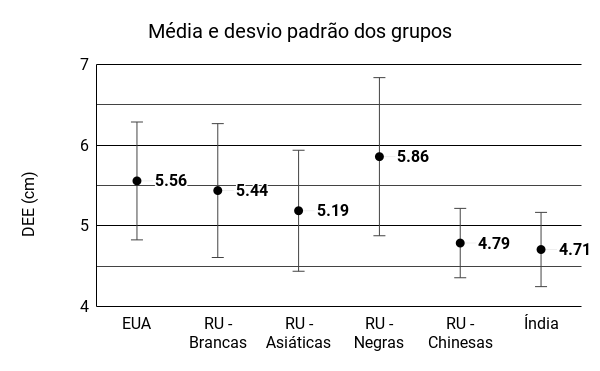
\includegraphics[width=0.9\linewidth]{capitulos/figuras/Media e desvio padrao dos grupos.png} 
    \caption{Média e desvio padrão da \acrshort{DEE} estimada pras populações de cada grupo de grávidas separadas pelo local dos estudos e grupos distintos }
    \label{fig:mediaDesvioPadraoPopulacoes}
\end{figure}

================================== artigo Anesthesua 1006 =====
Estimating population dat - Tabela 2
================================== 

A seguir iremos ilustrar parte da possibilidade de variabilidade de pacientes através dos parâmetros existentes no modelo 3D desenvolvido que pode ser alterado tanto via interface da \textit{Unity} como via código C\#. 

Como primeiro exemplo apresentamos a variabilidade de crescimento do tronco simulando uma paciente com um \acrshort{IMC} mais elevado em comparação com uma paciente com um corpo de \acrshort{IMC} mais baixo. As duas imagens apresentadas na Figura~\ref{fig:extremosCorpoIMC} ilustram os extremos que podem ser obtidos com a variação de parâmetros implementada no modelo 3D criado. Para variações maiores podemos usar transformações matriciais através de simples comandos na \textit{Unity} usando a transformação de escala aplicados. Optamos pela implementação de um range de variação para evitar a deformação por aplicações de matrizes de transformação que são aplicadas no objeto 3D como um todo. É sabido que existem regiões que são as mais afetadas pelo ganho de gordura corporal e, portanto devem ser mais expandidas do que outras visando um ganho visual mais próximo do real. Nestas figuras apresentamos o \texti{wireframe} de forma a ilustrar os polígonos que fazem parte do modelo 3D do corpo. Para fazer essas alterações via interface da \textit{Unity} primeiro é necessário importar o modelo 3D no projeto. Ele então precisa ser adicionado a hierarquia e ser corretamente posicionado na cena. Ao selecionar o elemento do modelo 3D (que neste caso se chama \textit{Body}) é preciso alterar o componente \textit{Skinned Mesh Renderer} associado pelo \textit{Unity} no momento da importação para cada camada (parte do modelo 3D) que possui parametrização (os componentes ficam na janela \textit{Inspector}). Este componente possui uma seção chamada \textit{BlendShapes} que exibe os parâmetros de deformação da forma. O parâmetro do objeto \textit{Body} se chama \textit{Body\_Final\_Channel} e aceita valores de zero a cem, sendo 0 (zero) o valor que indica a ausência de deformação (Figura~\ref{fig:extremosCorpoIMC} (a)) e 100 (cem) o valor de maior deformação (Figura~\ref{fig:extremosCorpoIMC} (b)). Para alteração via código na mudança de pacientes utilizamos o script em C\#. O acesso para modificação deste percentual de deformação é feito a partir da variável que representa o corpo, para este caso a camada chamada de \textit{Body} fica posicionada num vetor de camadas na primeira posição deste vetor. A Listagem~\ref{lst:codigo_alteracao_forma_paciente} apresenta um exemplo da parte do código que faz a deformação do corpo do paciente a partir do parâmetro passado. Este parâmetro é calculado como valor percentual a partir dos valores de \acrshort{IMC} mínimo e máximo implementados no sistema e do \acrshort{IMC} do paciente que é calculado a partir do seu peso e altura. Os valores mínimos e máximos de IMC são fixos pra cada execução do sistema sendo calculados a partir da base de pacientes disponível. Esta base pode ser alterada livremente para aumentar ou diminuir a variabilidade de cenários de teste conforme necessidade.

\begin{lstlisting}[label=lst:codigo_alteracao_forma_paciente, caption={Exemplo de alteração do corpo do paciente via script em C\#.}, language=sharpc]
float imc = objPaciente.peso / (objPaciente.altura * objPaciente.altura);

float percentDeformacaoCorpo = 100 * (imc - minIMC) / (maxIMC - minIMC);
        
SkinnedMeshRenderer smRenderer;
smRenderer = camadas[0].GetComponent<SkinnedMeshRenderer>();
smRenderer.SetBlendShapeWeight(0, percentDeformacaoCorpo);
\end{lstlisting}

\begin{figure}[ht!]
    \centering
        \begin{tabular}{cc}
        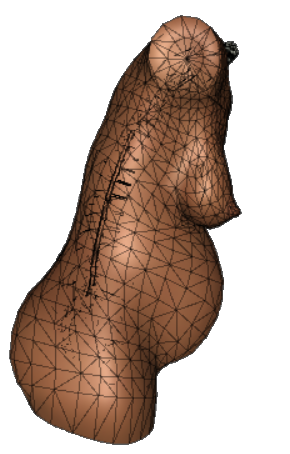
\includegraphics[width=0.4\linewidth]{capitulos/figuras/Corpo-menor-IMC-Wireframe.png} & 
        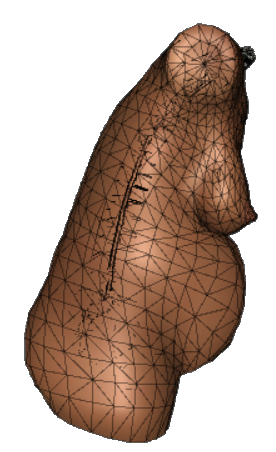
\includegraphics[width=0.38\linewidth]{capitulos/figuras/Corpo-maior-IMC-Wireframe.png} 
        \\
        (a) & (b)
        \end{tabular}
    \caption{Troncos com extremos de \acrshort{IMC} via parâmetro na posição lateral com \textit{wireframe}: (a) Menor \acrshort{IMC} (b) Maior \acrshort{IMC}.}
    \label{fig:extremosCorpoIMC}
\end{figure}

Na Figura~\ref{fig:pacientesMaiorParaMenorIMCVisaoTroncoELateral} exibimos todas as pacientes atualmente cadastradas no sistema ordenadas de forma decrescente em relação ao \acrshort{IMC}. Ao lado de cada tronco com os dados de idade, altura e peso inserimos também a visão lateral para melhor visualização das diferenças (que são distribuídas nos eixos X e Z). Fazendo um comparativo desde a paciente com maior \acrshort{IMC} (no alto a esquerda) até a de menor (abaixo a direita) é possível observar parte das variações implementadas no modelo 3D em relação a camada do corpo. Observando a área da cintura, barriga e dorso pode-se perceber o afinamento destas áreas conforme o \acrshort{IMC} é reduzido. É importante ressaltarmos aqui que a possibilidade de ajustar altura (crescimento no eixo Y) não foi trabalhada no modelo 3D por motivos de simplificação mas esta pode ser alterada a partir de transformações de matrizes via \textit{Unity}. O eixo mais importante para o contexto da simulação de raquianestesia é o da profundidade das camadas a serem transpassadas (eixo Z), por que é neste eixo que a agulha é inserida.

\begin{figure}[ht!]
    \centering
    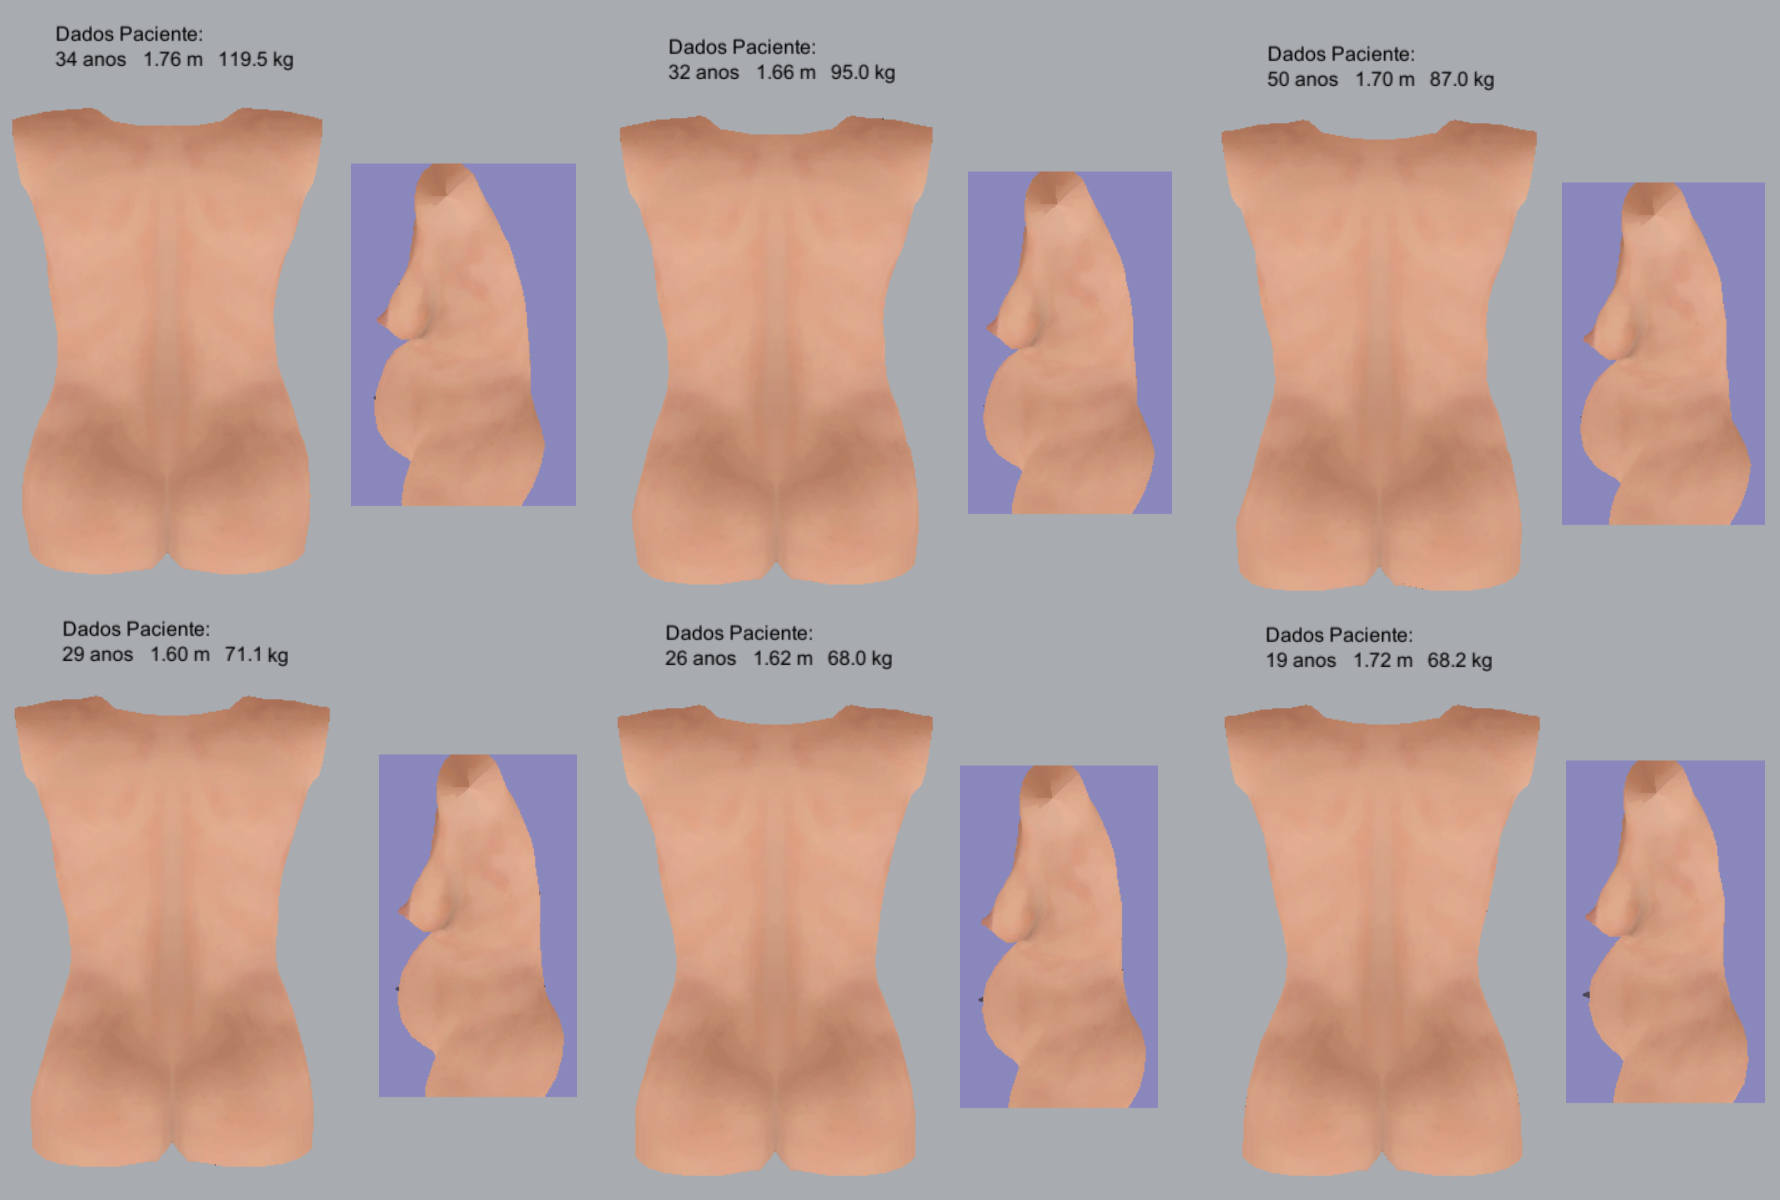
\includegraphics[width=0.9\linewidth]{capitulos/figuras/pacientes cadastradas maior para menor imc visao tronco sentado e lateral.png} 
    \caption{Ilustração dos troncos das pacientes cadastradas renderizados no sistema juntamente com a visão lateral do maior para o menor IMC.}
    \label{fig:pacientesMaiorParaMenorIMCVisaoTroncoELateral}
\end{figure}

Para configuração do \textit{Haptic Plug-In For Unity3D} \cite{Poyade2014} que é o plugin que utilizamos para tratar da interface entre dispositivo háptico com os itens 3D da simulação precisamos adicionar a cada camada do corpo alguns componentes. Os componentes a serem adicionados às camadas são o \textit{Haptic Properties} e o \textit{Mesh Collider} através da seleção da camada na hierarquia e, em seguida, no \textit{Inspector} deve-se ir no item Adicionar componentes e entrar com o nome destes. O componente \textit{Haptic Properties} vem junto com o \textit{Haptic Plug-In For Unity3D}. Ele serve para configurar as propriedades de interação com o háptico aos itens do universo 3D como as camadas do corpo da paciente no nosso caso (pele e demais camadas internas). Um exemplo de propriedade é a \textitr{Pop Through} que indica o quanto de força é necessário aplicar para que se perfure cada camada que está em contato com a agulha de anestesia durante uma simulação. Temos então configurações distintas para quando o movimento do háptico está representando o movimento do dedo do anestesista para apalpação e descobrimento do local correto de punção e para o momento que o movimento representa os objetos perfurantes como a seringa de anestesia local e a agulha de raquianestesia. No caso do anestesista estar fazendo a apalpação esta propriedade deve assumir um valor que desabilita a perfuração (o valor para este caso é zero). Demais características a respeito das propriedade utilizadas são descritas no capítulo~\ref{cap:cap5}. Já o componente \textit{Mesh Collider} é nativo do \textit{Unity} e é uma das formas de detecção de colisão da \textit{engine} que usa a geometria visível do objeto para tal. Outra configuração necessária para todos os objetos que tem interação com o háptico é a inclusão  da tag \textit{Touchable} que deve ser feita através do \textit{Inspector}. Esta também deve ser incluída em todos os objetos 3D que podem sofrer alguma influência a partir da movimentação do dispositivo háptico.

=== FALAR sobre associações de scripts Haptic Injection, GEneric Functions Class?